\documentclass[12pt]{article}

% math packages
\usepackage{amsmath, amsthm, amssymb, amsfonts}

% graphics packages
\usepackage{graphicx, subfigure}

% code packages
\usepackage{listings}

% language packages
\usepackage[italian]{babel}

% page geometry
\usepackage[a4paper, portrait, margin=0.85in]{geometry}

% links
\usepackage[colorlinks]{hyperref}

\usepackage{adjustbox}


\begin{document}

\title{
	Training an encoder-decoder with limited data for fetal femur segmentation from echographic images \newline
	\large Addestramento di un encoder-decoder per la segmentazione del femore fetale da immagini ecografiche}
\author{Ollari Ischimji Dmitri}

\maketitle

\newpage

\tableofcontents
\listoffigures
\listoftables

\newpage

%TODO:
% Introduzione dove spieghi un po' in generale il problema 
% che hai affrontato (segmentazione automatica di un oggetto
% su immagini di ecografie) e l'obiettivo.


\section{Introduzione}


\subsection{Binary Semantic Segmentation}

La segmantazione semantica è una tecnica di \textit{computer vision} che permette di assegnare ad ogni pixel di un'immagine un'etichetta che ne descrive il contenuto.

Nello specifico in questa tesi si tratta una sottocategoria della semganzione semantica,
ovvero la \textbf{Binary Semantic Segmentation}(segmentazione semantica
binaria), questa tecnica di \textit{computer vision} permette di assegnare ad ogni pixel di un'immagine un'etichetta che ne descrive il contenuto, ma a differenza della segmentazione semantica classica, che permette di assegnare ad ogni pixel una delle $N$ possibili etichette, la segmentazione semantica binaria permette di assegnare ad ogni pixel una delle due etichette possibili: \textbf{oggetto} o \textbf{sfondo}.

La segmentazione \`e una tipologia di problema molto ricorrente in ambito medico, in quanto permette di automatizzare alcune procedure che altrimenti sarebbero eseguite manualmente, riducendo i tempi di esecuzione e i costi,
permettendo di ottenere risultati pi\`u precisi e accurati limitando lo sforzo umano.


\subsection{Fully Convolutional Network}

Le \textbf{Fully Convolutional Network} (FCN) \cite{long2015fully} sono una tipologia di reti neurali convoluzionali (CNN) che permettono di effettuare segmentazioni semantice, in quanto sono in grado di gestire input di qualsiasi dimensione e di produrre mappe di segmentazione pi\`u precise grazie alla loro capacit\`a di apprendere contesti spaziali.

Le motivazioni riguardanti l'ampio utilizzo nel settore della \textit{computer vision}
sono legate all'assenza di strati completamente connessi (o lineari), che permettono di gestire l'intera immagine in una sola volta, piuttosto che suddividerla in regioni e processarle separatamente, rendendole pi\`u efficienti in termini di tempo di elaborazione e risorse computazionali,
questa caratteristica comporta anche una maggiore flessibilit\`a dell'input, in quanto non sono presenti strati completamente connessi che bloccano le dimensioni dell'input, e una maggiore tolleranza agli errori e al rumore, in quanto sono in grado di gestire errori e rumore nei dati di input, rendendole robuste in situazioni reali.
% di questa tipologia di reti neurali convoluzionali ricadono nella flessibilit\`a delle informazioni che \`e in grado di gestire, nella sua capacit\`a di generalizzazione e nella tolleranza agli errori e al rumore.

Nello specifico \`e stata utilizzata una architettura di rete neurale che prende il nome di \textbf{U-Net} \cite{ronneberger2015unet},
la scelta \`e ricaduta su questa architettura in quanto \`e stata progettata per lavorare con un numero ridotto di immagini di addestramento e produrre segmentazioni pi\`u precise.

% he U-Net architecture stems from the so-called “fully convolutional network” proposed by Long, Shelhamer, and Darrell in 2014.[2]
%
% The main idea is to supplement a usual contracting network by successive layers, where pooling operations are replaced by upsampling operators. Hence these layers increase the resolution of the output. A successive convolutional layer can then learn to assemble a precise output based on this information.[1]
%
% One important modification in U-Net is that there are a large number of feature channels in the upsampling part, which allow the network to propagate context information to higher resolution layers. As a consequence, the expansive path is more or less symmetric to the contracting part, and yields a u-shaped architecture. The network only uses the valid part of each convolution without any fully connected layers.[2] To predict the pixels in the border region of the image, the missing context is extrapolated by mirroring the input image. This tiling strategy is important to apply the network to large images, since otherwise the resolution would be limited by the GPU memory. 

L'architettura di tipo U-net rappresenta lo standard di riferimento per la segmentazione semantica di immagini biomediche, in quanto \`e in grado di gestire un numero ridotto di immagini di addestramento e produrre segmentazioni pi\`u precise.


% La rete neurale UNET è una rete neurale convoluzionale (CNN) sviluppata per la segmentazione di immagini biomediche1
% . È stata progettata per lavorare con un numero ridotto di immagini di addestramento e produrre segmentazioni più precise3
% . L'architettura di UNET è simmetrica e composta da due parti principali: un percorso di contrazione (o encoder) e un percorso di espansione (o decoder)3
% . Il percorso di contrazione è costituito da una tipica rete convoluzionale, mentre il percorso di espansione è costituito da strati convoluzionali trasposti 2D1
% . UNET è un esempio di Fully Convolutional Network (FCN), che significa che non ha strati completamente connessi (o lineari)5
% .


% Flessibilità dell'input: A differenza delle reti neurali convenzionali che hanno strati completamente connessi (fully connected layers) che bloccano le dimensioni dell'input, le FCN possono gestire input di qualsiasi dimensione. Questo è dovuto all'eliminazione del dense layer in favore di strati convoluzionali 1x1, che permette di superare le limitazioni delle reti neurali convenzionali2
% .
% Riduzione della perdita di informazioni: Durante il processo di down-sampling nell'encoder, le reti FCN gestiscono la perdita di informazioni ricostruendo l'immagine e recuperando parte delle informazioni dai filtri di pooling prima della sintesi dalla feature map3
% .
% Efficienza: Le FCN sono in grado di gestire l'intera immagine in una sola volta, piuttosto che suddividerla in regioni e processarle separatamente. Questo le rende più efficienti in termini di tempo di elaborazione e risorse computazionali1
% .
% Precisione: Le FCN sono in grado di produrre mappe di segmentazione più precise, grazie alla loro capacità di apprendere contesti spaziali a livello locale e globale1
% .
% Adattabilità: Le FCN sono adattabili a una varietà di applicazioni, tra cui la segmentazione di immagini, la classificazione di immagini e l'object detection4
% .
% Tolleranza agli errori e al rumore: Le FCN sono in grado di gestire errori e rumore nei dati di input, rendendole robuste in situazioni reali6
% .
% Capacità di aggiornamento: Le FCN possono essere facilmente aggiornate con nuovi dati, permettendo un apprendimento continuo e l'adattamento a nuove informazioni6
% .
% Capacità di generalizzazione: Le FCN sono in grado di generalizzare bene da un set di addestramento a dati non visti, rendendole utili per una varietà di compiti di apprendimento automatico6
% .
% Indipendenza da assunzioni a priori: A differenza di molti altri modelli di apprendimento automatico, le FCN non richiedono assunzioni a priori sui dati6
% .
% Applicabilità a problemi di regressione e classificazione: Le FCN possono essere utilizzate sia per problemi di regressione che di classificazione, rendendole versatili per una varietà di compiti6
% .

% Le motivazioni che hanno portato alla scelta di una rete di questo tipo ricadono
% nella flessibilità delle informazioni che è in grado di gestire, nella sua
% capacità di generalizzazione e nella tolleranza agli errori e al rumore.
%
% Nello specifico \`e stata utilizzata una architettura di rete neurale
% che prende il nome di \textbf{U-Net}. \cite{ronneberger2015unet}
%
%
%



% Fully convolution networks
%
% A fully convolution network (FCN) is a neural network that only performs convolution (and subsampling or upsampling) operations. Equivalently, an FCN is a CNN without fully connected layers.
% Convolution neural networks
%
% The typical convolution neural network (CNN) is not fully convolutional because it often contains fully connected layers too (which do not perform the convolution operation), which are parameter-rich, in the sense that they have many parameters (compared to their equivalent convolution layers), although the fully connected layers can also be viewed as convolutions with kernels that cover the entire input regions, which is the main idea behind converting a CNN to an FCN. See this video by Andrew Ng that explains how to convert a fully connected layer to a convolutional layer.
% An example of an FCN
%
% An example of a fully convolutional network is the U-net (called in this way because of its U shape, which you can see from the illustration below), which is a famous network that is used for semantic segmentation, i.e. classify pixels of an image so that pixels that belong to the same class (e.g. a person) are associated with the same label (i.e. person), aka pixel-wise (or dense) classification.


% Convolutional networks are powerful visual models that
% yield hierarchies of features. We show that convolu-
% tional networks by themselves, trained end-to-end, pixels-
% to-pixels, exceed the state-of-the-art in semantic segmen-
% tation. Our key insight is to build “fully convolutional”
% networks that take input of arbitrary size and produce
% correspondingly-sized output with efficient inference and
% learning. We define and detail the space of fully convolu-
% tional networks, explain their application to spatially dense
% prediction tasks, and draw connections to prior models. We
% adapt contemporary classification networks (AlexNet [19],
% the VGG net [31], and GoogLeNet [32]) into fully convolu-
% tional networks and transfer their learned representations
% by fine-tuning [4] to the segmentation task. We then de-
% fine a novel architecture that combines semantic informa-
% tion from a deep, coarse layer with appearance information
% from a shallow, fine layer to produce accurate and detailed
% segmentations. Our fully convolutional network achieves
% state-of-the-art segmentation of PASCAL VOC (20% rela-
% tive improvement to 62.2% mean IU on 2012), NYUDv2,
% and SIFT Flow, while inference takes less than one fifth of a
% second for a typical image.



\chapter{Lavori correlati} % (fold)
\label{chap:Lavori correlati}

% chapter Lavori correlati (end)
\section{Segmentazione ossea}


Un progetto degno di nota \`e \textbf{Towards whole-body CT Bone Segmentation} \cite{Klein_2018}
poich\`e si propone di risolvere il problema della segmentazione ossea di umani e la raggiunge con
ottimi risultati con accuratezza del $96\%\pm 2\%$ mediante la metrica di \textbf{Dice Score} e $94\%\pm 2\%$ con la metrica di \textbf{Intersection over Union}.


Il progetto si basa su una rete neurale convoluzionale che utilizza l'architettura U-Net \cite{ronneberger2015unet}
e raggiunge ottimi risulati con circa 4000 immmagini e 60 epoche di training lasciando
l'architettura della rete invariata.


\section{Segmentazione vasi sanguigni}
L'articolo \textbf{Accurate Retinal Vessel Segmentation via
Octave Convolution Neural Network} \cite{fan2019octave} propone un metodo di segmentazione automatico per la segmentazione dei vasi sanguigni retinici.

L'implementazione del metodo \`e basata su una rete neurale convoluzionale che utilizza l'architettura Octave UNet, modello che segue l'architettura di U-Net \cite{ronneberger2015unet} ma utilizza l'operazione di convoluzione octave e delle convoluzioni octave trasposte.

Le convoluzini octave sono state introdotte in \textbf{Drop an Octave: Reducing Spatial Redundancy in Convolutional Neural Networks with Octave Convolution} \cite{chen2019drop} e sono una variante delle convoluzioni standard che prova a ovviare al problema di sbilanciamento delle \textit{features} all'interno delle mappe di \textit{features}.






\chapter{Metodi} % (fold)
\label{chap:Metodi}

% chapter Metodi (end)
\section{Dati}

Tutti i dati provengono da analisi ecografiche effettuate presso \textbf{Azienda Ospedaliero-Universitaria di Parma}.
Le immagini raccolte si rifanno al periodo compreso tra \textbf{Aprile 2022} e \textbf{Gennaio 2023} e sono state selezionando tenendo conto di alcuni parametri per standardizzare l'input come:
\begin{itemize}
  \item Indice di massa corporea (BMI)
  \item Età delle madri
  \item Problematiche durante la gravidanza
  \item Problematiche dopo il parto
  \item Immagini scattate con la medesima angolazione rispetto al femore
\end{itemize}


Le immagini hanno subito un processo di \textit{preprocessing} aggiuntivo per uniformare le dimensioni e la risoluzione. In particolare, sono state ridimensionate a immagini \textbf{$1280px$ di larghezza} e \textbf{$876px$ di altezza}.


Inoltre data che il problema è categorizzato come problema di segmantazione semantica binomiale, si è scelto di convertire le immagine da \textbf{RGB} a immagini in \textbf{scala di grigi} per ridurre la complessità del problema e per ridurre il quantitativo di dati necessari per l'addestramento della rete.


Sono state realizzate manualmente delle \textbf{maschere} di segmantazione per ogni immagine, in modo da avere un \textit{ground truth} da confrontare con le predizioni del modello.


Data la scarsa quanti di dati a disposizione per l'addestramento della UNET, si è scelto di utilizzare alcune tecniche di \textit{data augmentation} per aumentare la quantità di dati a disposizione. In particolare si è scelto di utilizzare le seguenti tecniche applicate in modo casuale per ogni coppia \textbf{immagine-maschera}
\begin{itemize}
	\item \textit{Flip} orizzontale e verticale
	\item \textit{Rotazioni} di $35^{\circ}$
	\item \textit{Rumore} Gaussiano
\end{itemize}

Queste tecniche di \textit{data augmentation} migliorano notevolmente le segmentazioni ottenute mediante la rete UNET e rendono la rete più robusta a variazioni di luce e a rumore presente nelle immagini.


\begin{figure}[!ht]
	\begin{adjustbox}{width=0.95\columnwidth, center}
		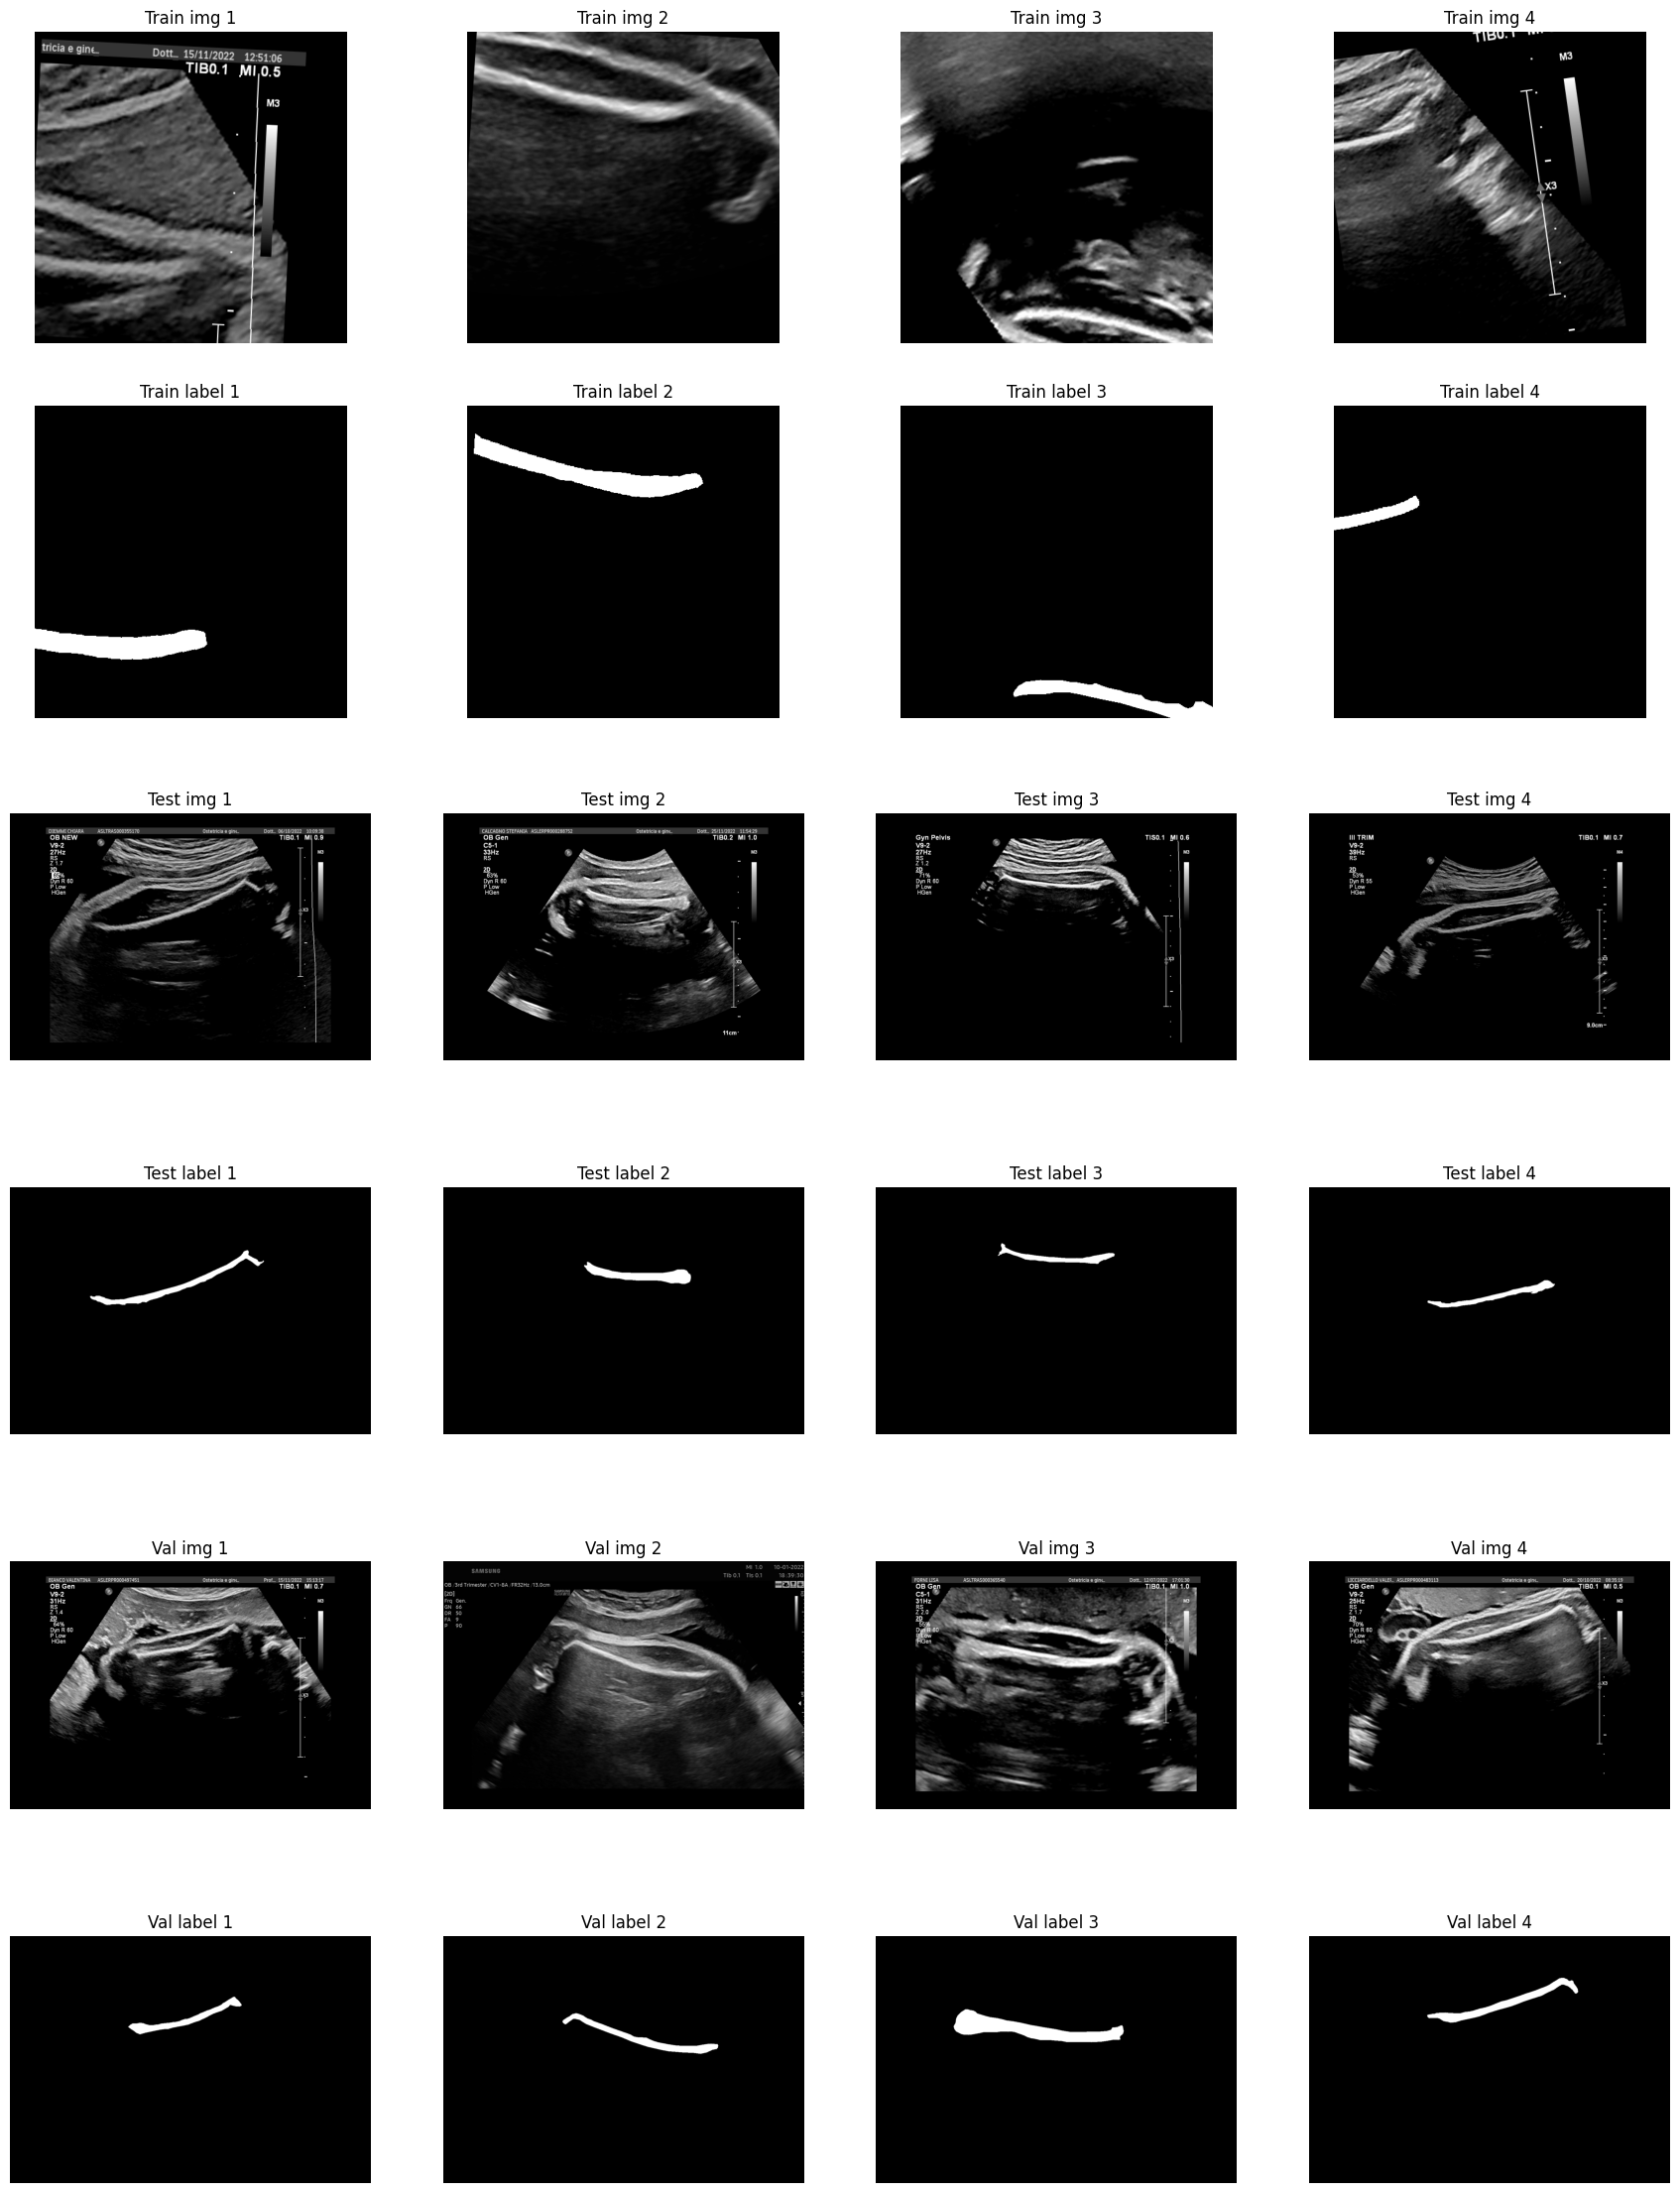
\includegraphics{./images/data_augmentation.png}
	\end{adjustbox}
  \caption{\textit{Data augmentation}}
  \label{fig:data_augmentation}
\end{figure}

L'ottimo risultato ottenuto è in buona parte dovuto alla \textit{data augmentation} effettuata nella fase di addestramento del modello, la \textit{data augmentation} ha migliorato l'adattabilità a contesti non controllati migliorando così la generalizzazione del modello.


Come si può notare dalla \autoref{fig:data_augmentation} la \textit{data augmentation} è stata effettuata in modo casuale per ogni coppia \textbf{immagine-maschera} ed è stata applicata solo nella fase di addestramento, lasciando cosi invariate le immagini inerenti al controllo del modello.




\section{Etichettatura}
Le immagini utilizzate per l'addestramento della rete sono state fornite da \textbf{Azienda Ospedaliero-Universitaria di Parma} e sono state etichettate manualmente mediante
l'uso di un software di etichettatura chiamato \textbf{LabelMe} \cite{labelme}.

Il processo di etichettatura della immagini prevede per ogni immagine l'applicazione di indicatori che delimitano il perimetro del femore, potendolo così isolare dal resto dell'immagine.


\section{Modello}

Il modello dal quale si è partiti prende il nome di \textbf{U-Net}(\autoref{fig:unet}), la sua realizzazione iniziale è stata effettuata seguendo lo studio di Olaf Ronneberger, Philipp Fischer e Thomas Brox del 2015 \cite{ronneberger2015unet}.

Lo studio propone un'architettura di rete neurale convoluzionale per la segmentazione semantica di immagini biomediche, classificando ogni singolo pixel dell'immagine in una delle varie categorie del problema analizzato, la rete convoluzionale emersa da quesa analisi rimane tutto'oggi una delle più utilizzate in ambito medico per la segmentazione semantica data la sue performace e la sua versatilità.

L'implementazione iniziale ricalca il modello realizzato da Olaf Ronneberger, Philipp Fischer e Thomas Brox, utilizzando il framework \textbf{PyTorch} \cite{pytorch} come base per la realizzazione della rete.

L'architettura proposta da Olaf Ronneberger, Philipp Fischer e Thomas Brox è composta di 4 parti principali:
\begin{itemize}
  \item \textbf{Encoder}: Visionabile graficamente come la parte discenente della U-Net
  \item \textbf{Bridge}: Visionabile graficamente come la linea di congiunzione fra la parte discendente e la parte ascendente della U-Net
  \item \textbf{Decoder}: Visionabile graficamente come la parte ascendente della U-Net
  \item \textbf{Output}: Visionabile graficamente come l'ultimo layer della U-Net
\end{itemize}

Le applicazioni che si appogiano a modelli derivati dall'architettura U-net dominano settori come la medicina e la biologia, in particolare la segmentazione di immagini biomediche, come la segmentazione di immagini ecografiche, la segmentazione di immagini TC e la segmentazione di immagini RM.

Le cause principali di tale successo possono essere ricondotte a:
\begin{itemize}
  \item \textbf{Segmentazione dettagliata}: U-Net è in grado di produrre segmentazioni dettagliate e precise grazie alle sue innovative "skip connections" che permettono al modello di catturare sia i dettagli di basso livello che il contesto di alto livello.
  \item \textbf{Architettura compatta}: Nonostante la sua capacità di catturare dettagli, il modello è relativamente snello e può essere addestrato con successo anche con dataset di dimensioni moderate.
  \item \textbf{Adattabilità}: U-Net è stata originariamente concepita per applicazioni mediche, ma si è dimostrata estremamente versatile e può essere utilizzata con successo in una vasta gamma di contesti.
\end{itemize}

Ovviamente, come ogni modello, U-Net ha anche alcuni svantaggi. Il principale è la necessità di un dataset di addestramento ampio e accuratamente etichettato. Questo aspetto può essere un ostacolo, soprattutto in contesti in cui la disponibilità di dati è limitata. Inoltre, U-Net richiede una quantità significativa di memoria per memorizzare i pesi del modello, il che può diventare un problema quando si lavora con immagini ad alta risoluzione.


\subsection{Convoluzione} % (fold)
\label{sec:convoluzione}


La convoluzione è una delle operazini fondamentali utilizzate nelle reti neurali convoluzionali per estrarre le caratteristiche significative da un'input, la convoluzione coinvolge un filtro (o kernel) e l'input su cui si applica.

Il processo di convoluzione consiste nell'sommare ogni elemento di un'immagine al suo vicino, pesando ogni singola operazione mediante l'utilizzo del filtro(o kernel) il calcolo della feature map di uscita è calcolata come segue:
\begin{align}
  &\Bigg( \begin{bmatrix}
    a & b & c \\
    d & e & f \\
    g & h & i
  \end{bmatrix}
  *
  \begin{bmatrix}
    1 & 2 & 3 \\
    4 & 5 & 6 \\
    7 & 8 & 9
  \end{bmatrix}
  \Bigg) [2, 2] =\\
  &= (i \cdot 1) + (h \cdot 2) + (g \cdot 3) + (f \cdot 4) + ( e \cdot 5 ) + ( d \cdot 6 ) + c \cdot 7) + (b \cdot 8) + (a \cdot 9)
\end{align}


% subsection convoluzionale (end)

\subsection{Max pooling} % (fold)
\label{sec:Max pooling}
Il \textit{max pooling} è un'operazione chiave all'interno della rete U-Net e delle reti neurali convoluzionali (CNN) in generale.

Il \textit{max pooling} è utilizzato per ridurre la dimensione delle feature map, consentendo di ridurre la complessità del problema da approssimare, comportando una maggior resistenza all'\textit{overfitting}, migliorando la capacit\'a di generalizzazione del modello e di ottenere una rappresentazione più invariante rispetto alle piccole variazioni spaziali nell'input.


% subsection Max pooling (end)

\subsection{Encoder} % (fold)
\label{sec:Encoder}

TODO: aggiungere immagini singole per i vari pezzi dell'encoder

La fase di \textit{encoding} è la prima fase della rete U-Net, composta da una serie di strati di convoluzione(\ref{sec:convoluzione}) e max pooling(\ref{sec:Max pooling}) che riducono progressivamente la dimensione spaziale dell'immagine mentre aumentano il numero di canali di \textit{features}.

Nello specifico, la fase di \textit{encoding} è composta da 3 parti principali:
\begin{itemize}
  \item \textbf{Strato iniziale}: Questo strato applica diverse operazioni di convoluzione ai dati di input per estrarre le caratteristiche di basso livello, come bordi e texture. Queste operazioni iniziali consentono al modello di comprendere dettagli fondamentali dell'immagine.
  \item \textbf{Downsampling}: Dopo lo strato iniziale, la fase di encoding utilizza operazioni di max pooling o convoluzione con un passo (stride) superiore a 1 per ridurre la dimensione delle feature map. Questo processo di downsampling riduce la risoluzione spaziale, ma aumenta il numero di canali delle feature, catturando informazioni di livello superiore. Ogni strato di downsampling estrae caratteristiche sempre più astratte e globali dall'immagine.
  \item \textbf{Strati intermedi}: Nel cuore della fase di encoding si trovano gli strati intermedi. Questi strati applicano operazioni di convoluzione multiple con l'obiettivo di catturare caratteristiche di complessità crescente. A ogni strato intermedio, le feature map si allargano, consentendo al modello di comprendere dettagli più ampi e contestuali. Questi strati intermedi sono cruciali per l'acquisizione di informazioni di alto livello.
\end{itemize}

% subsection Encoder (end)


\subsection{Bridge} % (fold)
\label{sec:Bridge}
Il \textit{bridge} è un'innovazione dell'architettura U-Net che contribuisce in modo significativo alla precisione della segmentazione delle immagini.

La fase di \textit{bridge} permette di trasferire informazioni rilevanti tra l'encoder e il decoder attraverso skip connections, che consentono il trasferimento di informazioni rilevanti. Questo approccio multi-scala è fondamentale per ottenere una segmentazione precisa delle immagini, poiché consente al modello di considerare dettagli sia di basso che di alto livello durante il processo di segmentazione.



% subsection Bridge (end)

\subsection{Decoder} % (fold)
\label{sec:Decoder}

Nella rete U-Net, la fase di decoding \'e responsabile della ricostruzione dell'immagine segmentata a partire dalle informazioni estratte durante l'encoding. Questa fase \'e fondamentale per ottenere una segmentazione di alta qualit\'a.

Le fasi principali del \textit{decoder} sono:
\begin{itemize}
  \item \textbf{Upsampling}: La fase di decoding inizia con l'operazione di upsampling, che serve a ripristinare gradualmente la dimensione delle feature map ai livelli originali dell'immagine. Ciò viene fatto utilizzando operazioni come la trasposta della convoluzione (deconvoluzione) o l'interpolazione bilineare. L'obiettivo è ottenere feature map di dimensioni compatibili con quelle dell'immagine di input.
  \item \textbf{Skip Connections}: Un aspetto distintivo della U-Net sono le skip connections, o connessioni di salto. Queste connessioni collegano le feature map estratte durante l'encoding alle corrispondenti feature map nella fase di decoding. Ciò consente di combinare informazioni multi-scala, in modo che il modello possa accedere sia a dettagli fini che a contesto di alto livello. Le skip connections sono fondamentali per migliorare la precisione della segmentazione.
  \item \textbf{Convoluzione nel Decoding}: Dopo l'upsampling e l'integrazione delle skip connections, vengono applicate operazioni di convoluzione per raffinare ulteriormente le feature map. Queste convoluzioni possono avere lo scopo di "mescolare" le informazioni o di catturare dettagli specifici a livelli più alti.
\end{itemize}

% subsection Decoder (end)

\subsection{Output} % (fold)
\label{sec:Output}
La parte finale della rete U-Net \'e composta da uno o più strati di convoluzione che riducono la profondità delle feature map alla dimensione desiderata per l'output finale. Questi strati producono l'immagine segmentata in cui ogni pixel è etichettato con la classe di appartenenza (esempio: sfondo, oggetto, ecc.).

% subsection Output (end)

\section{Rimozione sliding window} % (fold)
\label{sub:Rimozione sliding window}
Grazie agli avanzamenti tecnologici portati avanti negli anni da costruttori hardware e software, si è riusciti a ridurre notevolmente i tempi di elaborazione delle immagini e la grandezza massima delle immagini che possono essere elaborate.

Si è quindi scelto di rinunciare all'approccio sliding window che risulta più conservativo in termini di memoria e di tempo di elaborazione, per un approccio più moderno che sfrutta la potenza di calcolo delle GPU e la loro memoria dedicata notevolmente più grande rispetto alle GPU del passato.

Un \textit{effetto collaterale} riscontrato con l'utilizzo di immagini intere è quello della miglior comprensione spaziale delle immagini da parte della rete, questo effetto è dovuto al fatto che la rete ha a disposizione l'intera immagine e non solo una parte di essa, questo permette alla rete di comprendere meglio il contesto spaziale dell'immagine e di migliorare la segmentazione.

% section Rimozione sliding window (end)


\section{Modifica encoding e decoding} % (fold)
\label{sub:Modifica encoding e decoding}
Mediante svariate prove si è notato che aumentando il numero di iterazioni di convoluzione nei vari strati di encoding e decoding, si ottengono risultati migliori in termini di segmentazione a scapito di un aumento del tempo di elaborazione e del consumo di memoria.

Si è quindi scelto di modificare le fasi di \textit{decoding} e di \textit{encoding}:


\begin{table}[!ht]
	\begin{adjustbox}{width=\columnwidth,center}
		\begin{tabular}{cc}
			\begin{tabular}{|c|c|c|}
				\hline
				\textbf{Layer} & \textbf{In channels} & \textbf{Out channels} \\
				\hline
				\hline
				Encoder        & 1                    & 64                    \\
				\hline
				Encoder        & 64                   & 128                   \\
				\hline
				Encoder        & 128                  & 256                   \\
				\hline
				Encoder        & 256                  & 512                   \\
				\hline
			\end{tabular}
			 &
			\begin{tabular}{|c|c|c|}
				\hline
				\textbf{Layer} & \textbf{In channels} & \textbf{Out channels} \\
				\hline
				\hline
				Decoder        & 1024                 & 512                   \\
				\hline
				Decoder        & 512                  & 256                   \\
				\hline
				Decoder        & 256                  & 128                   \\
				\hline
				Decoder        & 128                  & 64                    \\
				\hline
			\end{tabular} \\
		\end{tabular}
	\end{adjustbox}
	\caption{Encoding e Decoding originale}
	\label{tab:encoding_originale}
\end{table}

\begin{table}[!ht]
	\begin{adjustbox}{width=\columnwidth,center}
		\begin{tabular}{cc}
			\begin{tabular}{|c|c|c|}
				\hline
				\textbf{Layer} & \textbf{In channels} & \textbf{Out channels} \\
				\hline
				\hline
				Encoder        & 1                    & 16                    \\
				\hline
				Encoder        & 16                   & 32                    \\
				\hline
				Encoder        & 32                   & 64                    \\
				\hline
				Encoder        & 64                   & 128                   \\
				\hline
				Encoder        & 128                  & 256                   \\
				\hline
				Encoder        & 256                  & 512                   \\
				\hline
			\end{tabular}
			 &
			\begin{tabular}{|c|c|c|}
				\hline
				\textbf{Layer} & \textbf{In channels} & \textbf{Out channels} \\
				\hline
				\hline
				Decoder        & 1024                 & 512                   \\
				\hline
				Decoder        & 512                  & 256                   \\
				\hline
				Decoder        & 256                  & 128                   \\
				\hline
				Decoder        & 128                  & 64                    \\
				\hline
				Decoder        & 64                   & 32                    \\
				\hline
				Decoder        & 32                   & 16                    \\
				\hline
			\end{tabular} \\
		\end{tabular}
	\end{adjustbox}
	\caption{Encoding e Decoding modificati}
	\label{tab:encoding_modificato}
\end{table}

L'idea alla base di questa modifica risiede nel significato intrinseco dell'operazione di convoluzione e di max pooling, 
aggiungendo iterazioni di convoluzioni, si permette alla rete in primo 
luogo di estrarre più feature importanti alla classificazione dei pixel e successivamente mediante il max pooling
si eliminano le feature meno importanti e si riduce la dimensione delle feature map.



% section Modifica encoding e decoding (end)



\section{Metriche}

Considerando la tipologia di \textit{task} si è pensato di usare la metrica \textit{Dice BCE Loss} per la \textit{loss} e \textit{Intersection over Union} per l'\textit{accuratezza}.

\subsection{Dice BCE Loss}
La \textit{Dice BCE Loss} è una metrica che combina due metriche, la \textit{Dice Loss} e la \textit{BCE Loss}.

\begin{align}
	% \text{DiceBCELoss} &= \text{DiceLoss} + \text{BCELoss}
	L & = L_{\text{Dice}} + L_{\text{BCE}}
	\label{eq:dice_bce_loss}
\end{align}

\begin{align}
	L_{\text{Dice}} & = 1 - \frac{2\sum_i^N p_i g_i + \varepsilon}{\sum_i^N p_i^2 + \sum_i^N g_i^2 + \varepsilon}
	\label{eq:dice_loss}
\end{align}

\begin{align}
	L_{\text{BCE}} & = -\frac{1}{N} \Bigg[ g_i \sum_{i=1}^N p_i + ( 1 - g_i ) \sum_{i=1}^N (1-p_i) \Bigg]
	\label{eq:bce_loss}
\end{align}

Quindi ne risulta che la \textit{loss} sarà calcolata mediante:
\begin{align}
	L & = 1 - \frac{2\sum_i^N p_i g_i + \varepsilon}{\sum_i^N p_i^2 + \sum_i^N g_i^2 + \varepsilon} -\frac{1}{N} \Bigg[ g_i \sum_{i=1}^N p_i + ( 1 - g_i ) \sum_{i=1}^N (1-p_i) \Bigg]
	\label{eq:dice_bce_loss_complete}
\end{align}
Dove:
\begin{itemize}
	\item $p_i$ è il valore di \textit{ground truth}
	\item $g_i$ è il valore \textit{predetto} dal modello
\end{itemize}

\subsection{Intersection over Union(IoU)}
Per la metrica dell'accuratezza della segmentazione, è stata utilizzata la metrica \textit{Intersection over Union} (IoU),
poichè è una metrica che permette di valutare la capacità di segmentazione del modello
facendo il rapporto tra l'area di intersezione tra la maschera predetta e quella di \textit{ground truth} e l'area di unione tra le due maschere, formalmente:
\begin{align}
	\text{IoU} & = \frac{\text{TP}}{\text{TP} + \text{FP} + \text{FN}}
	\label{eq:iou}
\end{align}

Dove \textbf{TP} è il numero di \textit{True Positive}, \textbf{FP} è il numero di \textit{False Positive} e \textbf{FN} è il numero di \textit{False Negative}.

\section{Validazione del modello}

La \textit{cross-validation} (validazione incrociata) è una tecnica fondamentale nell'ambito del machine learning e dell'addestramento di modelli predittivi. Essenzialmente, la cross-validation è un metodo per valutare le prestazioni di un modello in modo robusto, valutandolo su più insiemi di dati per ottenere stime più affidabili delle sue capacità predittive. Questo processo aiuta a mitigare il rischio di overfitting (sovradattamento) e offre una migliore comprensione delle prestazioni del modello.

\begin{figure}[!ht]
	\begin{adjustbox}{width=0.7\columnwidth, center}
		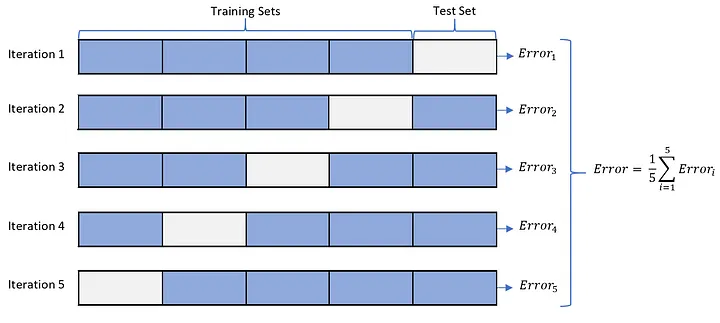
\includegraphics{./images/cross_validation.png}
	\end{adjustbox}
  \caption{Cross-validation}
  \label{fig:cross_validation}
\end{figure}

Fornisce stime più affidabili delle prestazioni del modello, riducendo il rischio di ottenere stime di prestazioni spurie a causa di una singola divisione dei dati.




\newpage
\bibliographystyle{plain}
\bibliography{bibliography}
\end{document}
